\chapter{Desarrollo del proyecto\label{sec:disenho}}

Para la realización de este trabajo se han tomado dos de las tecnologías expuestas en el capítulo \ref{sec:estado_del_arte} y se han llevado a la práctica. De esta manera se puede trabajar empíricamente con dos tecnologías diferentes planteadas como solución para un mismo problema. Una vez realizado todo el trabajo experimental se puede proceder a evaluar las características prácticas de cada tecnología y compararlas entre ellas. 

En función de la tecnología en que la se apoya cada uno de las soluciones, %por un lado se estudian los sensores de fibra FBG, capítulo \ref{sec:FBG3}, y por otro lado, los sensores IMU, capítulo \ref{sec:IMU3}.  
este capítulo se estructura de la siguiente manera: 
\begin{itemize}
	\item {\textbf{\ref{sec:FBG3}}    .- Solución con sensores de fibra FBG} 
	\item {\textbf{\ref{sec:IMU3}}    .- Solución con sensores IMU}
\end{itemize}




Dentro de cada punto se detalla toda la información necesaria para la implementación de cada uno de los sistemas. En ambos casos, la exposición de la solución tomada se divide en la explicación teórica en el \textit{Marco conceptual} y el ensayo práctico en el \textit{Desarrollo del prototipo}. El desarrollo del prototipo estudia los materiales empleados, el proceso de fabricación y el funcionamiento.  

%------------------------------
%------___SOLUCIÓN_FBG___------
%------------------------------
\section{Solución con sensores de fibra FBG}
\label{sec:FBG3}

\textcolor{rositaoscuro}{
	\textit{
		\colorbox{yellow}{Introducción} breve del guante, que tecnologias implica.
		Resumen fibras de Bragg 
		¿Qué es una fibra FBG?
		¿Porque se utilizan?
		El procesado de las señales resultantes se realiza mediante Labview.
	}
}


 Como primer prototipo se ha estudiado y llevado a cabo un guante cuyo funcionamiento se basa en los sensores de fibra FBG. 
 
 El prototipo consiste en una sección de PDMS con forma de huella de mano que tiene embebida una red en fibra de Bragg. Para la obtención, procesado y visualización de los resultados medidos se emplea el entorno de desarrollo LabVIEW.


%--Marco conceptual
\subsection{Marco conceptual}
\label{sec:mc3FBG}

Este apartado tiene por finalidad realizar una clara exposición de los conceptos teóricos fundamentales para la comprensión del diseño llevado a cabo. 

\begin{itemize}
%--FIBRA ÓPTICA
	\item \textbf{Fibra óptica}
	
	\textcolor{rositaoscuro}{
		\textit{
			- -Cómo se propaga la luz en ella.\\
	 		- -Partes de la fibra.\\
			Tipos de emisores (LED Laser).\\
			Receptores.\\
			Conectores y soldaduras.\\
			- -Fabricación.\\
			- -Tipos de fibra.\\
		}
	}

	%-- ¿Qué es la fibra óptica y la comunicación óptica?
	La fibra óptica es una hebra de material dieléctrico, así cómo el vidrio (sílice) o el polímero acrílico. 
	Se emplea como medio de propagación de señales luminosas. Es decir, para transmitir ondas electromagnéticas del espectro óptico: regiones espectrales de infrarrojo, luz visible y ultravioleta. En la siguiente imagen (figura \ref{fig:espectroOptico}) se puede observar dentro del espectro electromagnético dónde se sitúa el espectro óptico.	 
	
	\begin{figure}[H]
		\centering
		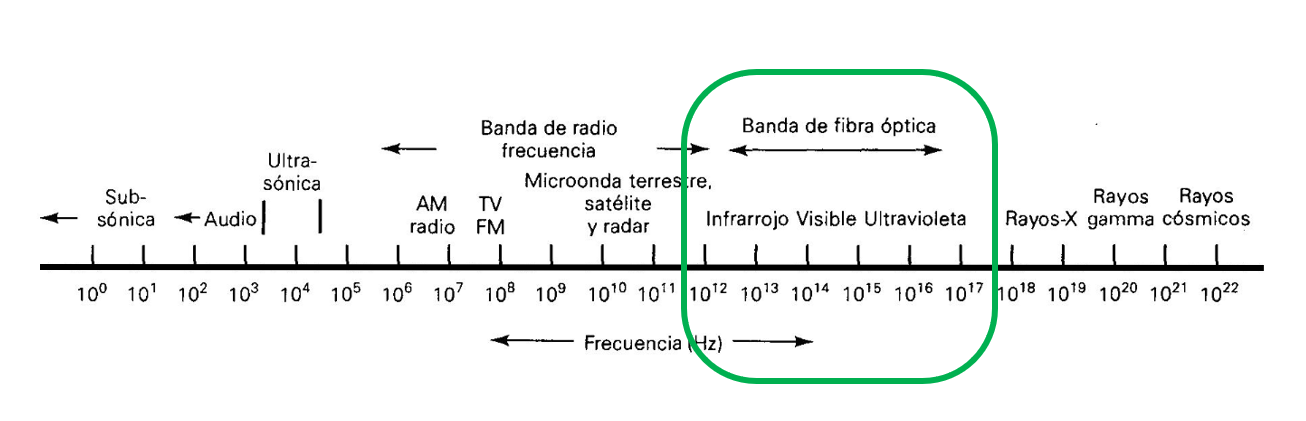
\includegraphics[width=0.95\textwidth]{./img/espectrooptico}
		\caption{Espectro electromagnético en frecuencia.}
		\label{fig:espectroOptico}
	\end{figure}
	
	%--Ventanas de comunicación por FO
	Cabe destacar que dentro del espectro óptico las longitudes de onda habituales para comunicación en fibra óptica están entre los 700nm y 1600nm. Estas se dividen en rangos con mejores características para la transmisión, denominadas ventanas de comunicación. Como se muestra en la figura \ref{fig:ventanaOptica}, son tres las ventanas más utilizadas,\cite{ventanasFO}:
 	\begin{table}[H]
		%\centering
		\hspace{2cm}
		\renewcommand{\arraystretch}{2}
		\begin{tabular}{rrl}
			\textbf{1ª ventana}& 800 a  900 nm  & $\longmapsto$ $\,$ longitud de onda utilizada = 850nm  \\
			\textbf{2ª ventana}& 1250 a 1350 nm & $\longmapsto$ $\,$ longitud de onda utilizada = 1310nm  \\
			\textbf{3ª ventana}& 1500 a 1600 nm & $\longmapsto$ $\,$ longitud de onda utilizada = 1550nm   \\ 
		\end{tabular} 
	\end{table}

	 \begin{figure}[H]
	 	\centering
	 	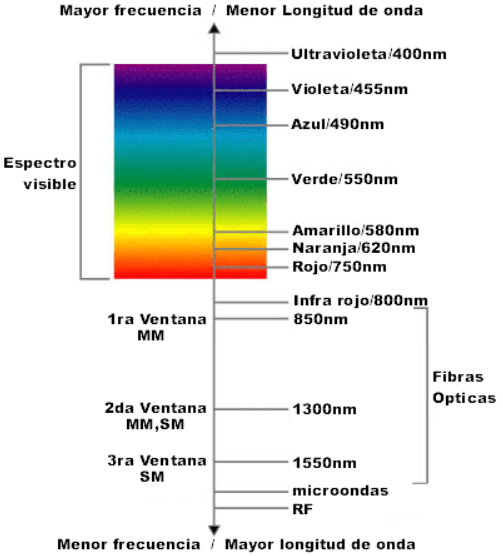
\includegraphics[width=0.5\textwidth]{./img/ventana}
	 	\caption{Longitud de onda fibra óptica junto con el espectro visible. \cite{ventanasFO}}
	 	\label{fig:ventanaOptica}
	 \end{figure}
 	La razón de que las ventanas de comunicación utilizadas se sitúen en las frecuencias indicadas reside en los diferentes comportamientos que tiene la atenuación de las señales en función de la longitud de onda (ver figura \ref{fig:perdidasFrec}). Existen algunas zonas dónde la atenuación es mínima, coincidiendo con la segunda y la tercera ventana. En cambio, en la zona correspondiente a la primera ventana las pérdidas no son mínimas, pero sí que se mantienen constantes. 	
 	
 	\begin{figure}[H]
 		\centering
 		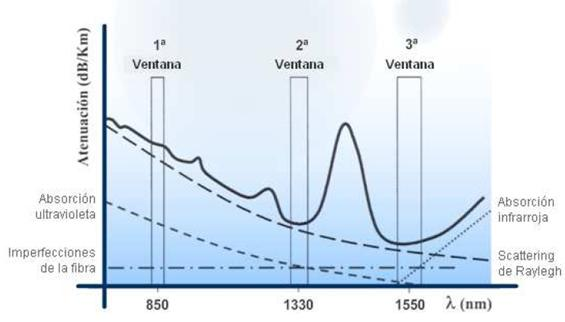
\includegraphics[width=0.8\textwidth]{./img/perdidasFrec}
 		\caption{Atenuación(dB/Km) frente a longitud de onda  $\lambda$ (nm) \cite{imgRadioModo}}
 		\label{fig:perdidasFrec}
 	\end{figure}

 %-- Características físicas de la fibra
 En cuanto a las propiedades físicas de la fibra óptica, son bastante delicadas ya que su grosor no supera por mucho al diámetro del cabello humano y se obtiene de la extrusión del sílice, SiO\textsubscript{2} , es decir, se trata de un filamento de vidrio muy fino. Es por ello que es la fibra óptica estándar está rodeada de una cubierta protectora. 
 
  \begin{figure}[H]
  	\centering
  	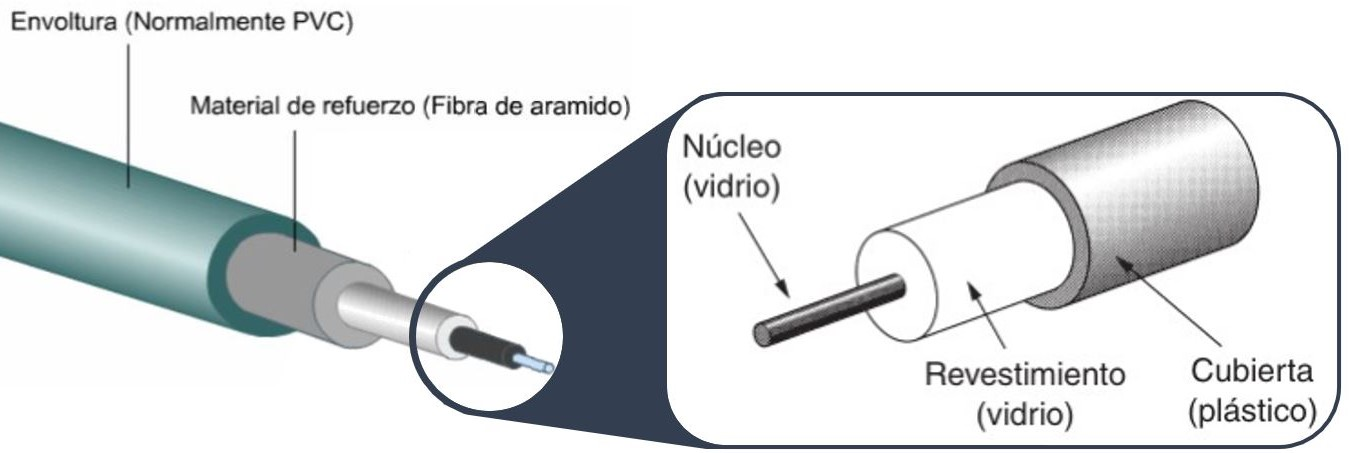
\includegraphics[width=0.87\textwidth]{./img/capas-fibra2}
  	\caption{Capas fibra óptica \cite{imgNucleoFibra,imgCapasFO}} 
  	\label{fig:capasFibra}
  \end{figure} 
  
  
  
 La fibra óptica estándar cuenta varias capas (figura \ref{fig:capasFibra}): núcleo, revestimiento y cubierta (o buffer).  Si la aplicación lo permite, conviene proteger la fibra con más capas externas. En la imagen anterior la fibra está además protegida por un material de refuerzo (fibra de aramido) y una envoltura (PVC).
 
 Tanto el núcleo cómo el revestimiento forman el medio por el cual se propaga la luz. Estas dos capas son tan finas que forman un filamento flexible, pero muy delicado, puesto que es muy propenso a romperse ante dobleces u otras manipulaciones externas. Por ello el resto de las capas son tambien importantes por proporcionar a la fibra protección y haciendo posible su utilización es escenarios de despliegue.
 
 %-- Fabricación FO
 La fabricación de la fibra óptica es un proceso de alta tecnología. Es importante mantener la pureza y la regularidad del núcleo. Esto es complejo, puesto que estamos hablando en algunos casos de núcleos de un grosor entorno a las 8 micras (en fibras monomodo). El grosor estándar de la fibra es de 125 micras(una micra equivale a una millonésima parte de un metro). Para conseguir este resultado el proceso de fabricación consiste en reproducir a escala macroscópica la estructura de la fibra que se quiere obtener. Esta reproducción a gran escala de la fibra deseada se le denomina preforma. Una vez se tiene la preforma, esta se va fundiendo y estirando hasta alcanzar el filamento del diámetro deseado. De una preforma se pueden sacar kilómetros de fibra. Para fabricar la preforma se parte de una barra de vidrio hueca (el vidrio que formará el recubrimiento) y se baña en un gas que contiene unas partículas (lo que formará el núcleo). Al calentar a mil grados, las partículas comienzan a fundirse hasta que el tubo colapsa y forma una vara maciza, que es la preforma. Para fundirla y estirarla esta se coloca verticalmente y se calienta. La complejidad de esta fase reside en mantener constante el flujo y el diámetro del hilo resultante. Además durante esta fase se aprovecha para crear una capa protectora sobre el vidrio (cubierta en la figura \ref{fig:capasFibra}). Finalmente los kilómetros de fibra óptica se enrollan en grandes bobinas. \cite{fabricacionFO}
 
 %-- Fibra Monomodo y multimodo
  \begin{figure}[H]
 	\centering
 	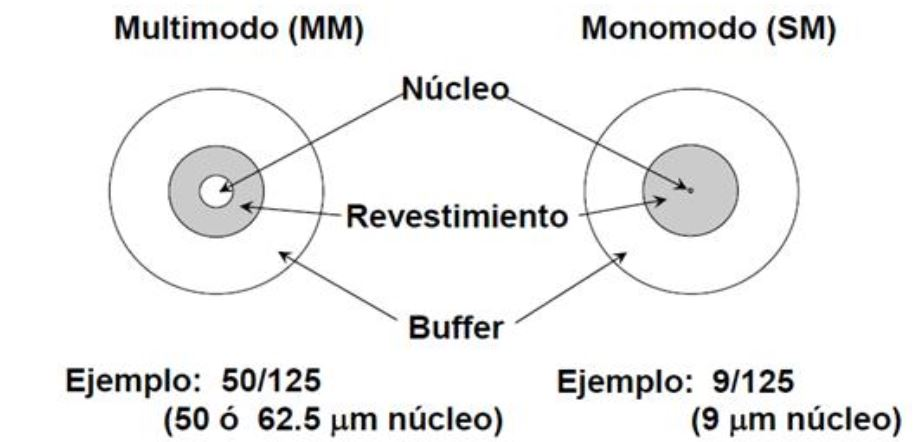
\includegraphics[width=0.6\textwidth]{./img/MM-SM}
 	\caption{Relación grosor fibra multimodo (MM) y monomodo (SM) \cite{imgRadioModo} } 
 	\label{fig:modoMonoMulti}
 \end{figure} 
 
  Dependiendo de la relación de diámetro entre el núcleo y el revestimiento, la fibra fibra será monomodo o multimodo (figura \ref{fig:modoMonoMulti}). Esta diferencia afecta a la propagación de la luz dentro de la guía de onda (figuras \ref{fig:guiaMM}, \ref{fig:guiaSM}, \ref{fig:indiceMultimodo}). Ya se ha comentado que el diámetro de la fibra es de aproximadamente 125 micras. En el caso de las fibras monomodo, el núcleo de estas tiene un diámetro tan pequeño (en torno a 8 micras) que la luz solo puede propagarse en un sólo modo (rayo). Sin embargo, en el caso de las fibras multimodo, al poseer un núcleo mayor (entre 50 o 62.5 micras) soportan la transmisión el múltiples modos, es decir, los rayos de luz viajan en muchas direcciones a través de este. \cite{FOA} 
   
   	\begin{figure}[H]
		\centering
		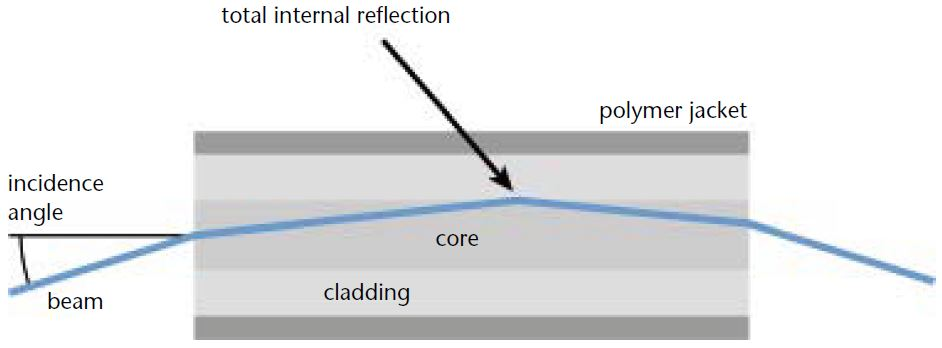
\includegraphics[width=0.7\textwidth]{./img/guiaMM}
		\caption{Corte transversal fibra multimodo en transmisión de luz. \cite{imgMonoMulti} } 
		\label{fig:guiaMM}
	\end{figure} 
  	\begin{figure}[H]
		\centering
		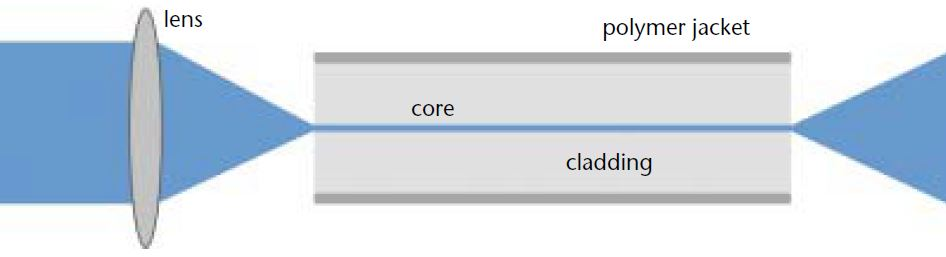
\includegraphics[width=0.7\textwidth]{./img/guiaSM}
		\caption{Corte transversal fibra monomodo en transmisión de luz. \cite{imgMonoMulti} } 
		\label{fig:guiaSM}
	\end{figure}  
 	
 	%-- Relación monomodo y multimodo con las longitudes de onda
 	Relacionando los tipos de fibras ópticas con las ventanas en las que trabajan, las fibras multimodo suelen trabajar en primera y segunda ventana, mientras que las fibras monomodo en segunda y tercera. 

	  	\begin{figure}[H]
		\centering
		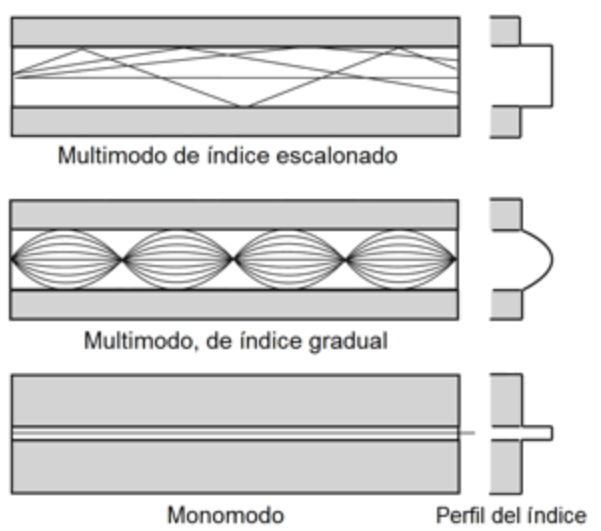
\includegraphics[width=0.5\textwidth]{./img/transFO-esc-grad}
		\caption{Disposición rayos. Multimodo (indice escalonado y gradual) y monomodo. \cite{FOA} } 
		\label{fig:indiceMultimodo}
		\end{figure}
	
 	%-- Otros tipos de FO
 	Además existen otros tipos de fibras menos comunes: la fibra de plástico (POF) y la fibra de sílice con revestimiento de plástico (HCS/PCS). La primera tiene un núcleo de gran diámetro ($1mm$ aproximadamente), puede utilizarse para redes de distancia corta y de baja velocidad. Las fibras de sílice con revestimiento de plástico tienen un núcleo más pequeño ($200\mu m$ aproximadamente) que las fibras de plástico. Estos dos últimos tipos de fibra multimodo generalmente son de índice escalonado, mientras que el resto de fibras multimodo suelen ser de índice gradual. En la figura \ref{fig:indiceMultimodo} se observa como es la diferencia en la distribución de los rayos en un caso y en el otro. En cuanto al tamaño de las fibras, la figura \ref{fig:otrosTiposFO} se representan las diferentes relaciones de tamaños entre los cinco tipos de fibra vistos. \cite{FOA}
 	 	
 	 \begin{figure}[H]
 	 	\centering
 	 	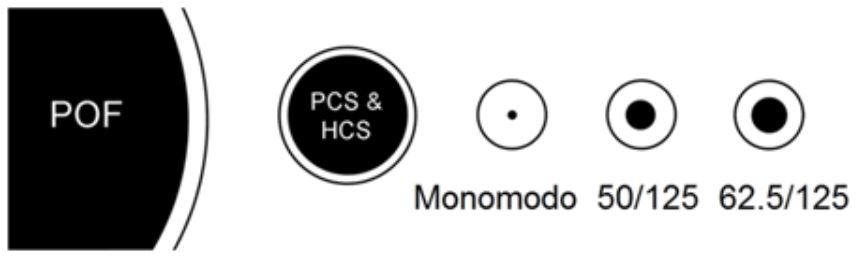
\includegraphics[width=0.7\textwidth]{./img/tiposFO}
 	 	\caption{Relación tamaños fibras ópticas. \cite{FOA} } 
 	 	\label{fig:otrosTiposFO}
 	 \end{figure} 	
  	
 %-- PROPAGACIÓN DE LA LUZ	
 %-- Diferenci de indices de refracción
 La diferencia de índices de refracción entre las capas centrales de la fibra son las que permiten la propagación de la luz a través de esta. El núcleo tiene un mayor indice de refracción que el revestimiento, lo que genera que los rayos de luz se curven a medida que pasan del núcleo al revestimiento, generando una "reflexión interna total" en la fibra. La siguiente imagen (figura \ref{fig:TIR}) sirve para explicar claramente este concepto:
 
 \begin{figure}[H]
 	\centering
 	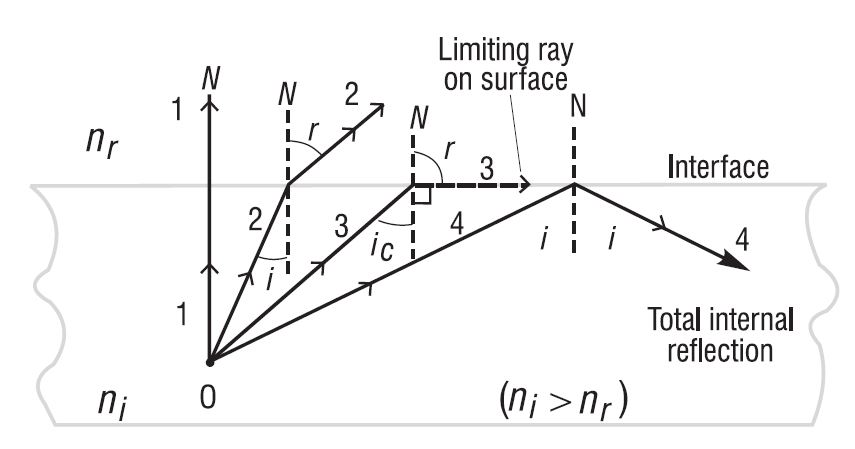
\includegraphics[width=0.66\textwidth]{./img/TIR}
 	\caption{Ángulo crítico y reflexión interna total. \cite{geometriaBasicaFP} } 
 	\label{fig:TIR}
 \end{figure}
 
 %Reflexión interna total
 En la figura \ref{fig:TIR} se ilustran cuatro rayos que se originan en el puno 0, lo que sería el núcleo de la fibra óptica (dónde el indice de refracción \textit{n\textsubscript{i}} es mayor). Entre los cuatro rayos varía el ángulo con el que estos inciden sobre el revestimiento (de menor índice de refracción\textit{n\textsubscript{r}}). Se observa cómo en el rayo número 1 incide con $90\,^{\circ}$ (incidencia normal), no habiendo reflexión y siguiendo el rayo en la misma dirección. En el rayo número 2 incide con un ángulo \textit{i}, y se refracta con \textit{r}. El rayo número 3 incide con el ángulo crítico \textit{i\textsubscript{c}}, suficientemente grande para que el rayo reflejado se propague a lo largo de la interfaz entre los dos medios, quedando atrapado. Por último, el rayo número 4 incide con un ángulo \textit{i} superior al ángulo crítico (ecuación \ref{eq:angCritico}), \textit{i\textsubscript{c}}, consiguiendo que se refleje totalmente en el mismo medio del que incide. Este rayo obedece a la ley de reflexión, siendo su ángulo de reflexión exactamente igual a su ángulo de incidencia. Este fenómeno se denomina \textit{"Reflexión interna total"}, necesario para que suceda la transmisión de señales lumínicas en la fibra óptica. 

	\begin{equation}
		\label{eq:angCritico}
		\hat{i}\textsubscript{c} =  \sin^{-1}\left(\dfrac{n\textsubscript{r}}{n\textsubscript{i}}\right)
	\end{equation}

 La reflexión interna total atrapa la luz hasta cierto ángulo en el núcleo, definiendo la apertura numérica a la que hay que asegurarse de penetrar la luz para que se de el fenómeno de reflexión interna total. Así se fuerza a que la mayoría de los rayos de luz incidan sobre el interfaz y se reflejen, permitiendo la transmisión de la señal lumínica. 
 
 
 
 \textcolor{rositaoscuro}{//----------------------------------------------------------------------- }\\ 
 %No vamos a hablar más de multimodo
 (\\Puesto que en la solución llevada a cabo en este trabajo se utilizan fibras monomodo no se va a extender el texto en explicar más conceptos sobre la transmisión en fibras multimodo.\\)\\
 \textcolor{rositaoscuro}{-------------------------------------------------------------------------//}\\
 
 
 %Sistemas de propagación
   \begin{figure}[H]
 	\centering
 	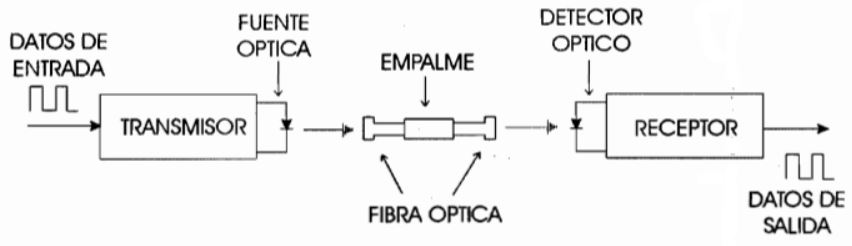
\includegraphics[width=1\textwidth]{./img/TxFOp2p}
 	\caption{Transmisión punto a punto de señales a través de fibra óptica. \cite{txFO} } 
 	\label{fig:TxFOp2p}
 \end{figure} 
 
 Los sistemas de propagación de señales luminosas a través de la fibra óptica componen un medio de transmisión de datos rápido y fiable. En la figura \ref{fig:TxFOp2p} se plasma el procedimiento que sigue la transmisión de datos en un sistema óptico y los elementos que lo componen. Previa a la propagación a través de un medio óptico de una señal eléctrica (analógica o digital) es necesario realizar una conversión de esta a señal óptica. Esto genera una señal óptica a partir de una señal eléctrica en el emisor o fuente de luz situado en el extremo inicial de la comunicación. Realizada la conversión, la señal es transmitida a lo largo de la fibra óptica. Según las características del escenario puede haber una o varias uniones entre fibras a lo largo del canal. Estás pueden realizarse empalmando o utilizando conectores. Una vez la señal óptica atraviesa todo el canal, llega al detector, dónde sucede el proceso inverso al ocurrido en el emisor y a la salida del sistema completo se tiene la señal eléctrica. Esta corresponde a la señal introducida al sistema con una pequeña posibilidad de haber sufrido pérdidas o atenuación debido a la impureza de la fibra, la distancia, las conexiones entre elementos del sistema o cualquier otro evento ajeno al este. Estas modificaciones de la señal de entrada pueden ser contrarrestadas o solventadas en recepción sin suponer un impedimento a una comunicación exitosa.    
  
 Veamos por separado los elementos dibujados en la figura \ref{fig:TxFOp2p}:
 	\begin{itemize}
 		\item \textit{\textbf{Emisores (Transmisión)}}	
 		% \hspace{0.2cm} 
 		
 		//--Los emisores de luz son los responsables de la conversión de la señal eléctrica en señal luminosa antes de su propagación a través de la fibra. Un emisor se puede dividir en dos partes.
 		//--En primer lugar, se considera la propia fuente de luz y, en segundo lugar, el dispositivo que controla la potencia de la fuente de emisión. Según la forma de generar los fotones, las fuentes más empleadas para la emisión de luz son los diodos LED y los láseres.
 		
 		//---LED
 		//Los diodos emisores de luz conocidos como LED (Light Emitting Diodes), son las fuentes más simples y baratas para la emisión de luz en el interior de la fibra óptica. Son un elemento semiconductor que emite luz en un espectro reducido cuando se polariza y se le hace circular corriente eléctrica. Las longitudes de onda de emisión de un diodo LED pueden variar desde el ultravioleta hasta el infrarrojo, dependiendo del material semiconductor con el que se fabrique.
 		//Entre sus principales ventajas destacan la baja potencia de alimentación, gran tiempo de vida y la posibilidad de fabricar un elevado número de dispositivos [22]. Estas ventajas reducen su coste y permiten configurar elementos de menor tamaño. Además, posee un espectro de emisión más amplio que los diodos láser (Fig. 3.4.). Sin embargo, es de gran dimensión	respecto a la relación de tamaño con la fibra, por tanto, solo lo hacen adecuado para las fibras en régimen multimodo.
 		//---Láser
 		//Los láseres (Light Amplification by Stimulated Emission of Radiation) son las fuentes ópticas con mayor capacidad de transmisión de la luz a lo largo de la fibra. Estos emisores concentran la luz en forma de haces muy pequeños pero potentes, de forma que su radiación es muy direccionada e intensa (Fig. 3.4.). Esto origina un espectro más estrecho con una gran potencia óptica de emisión [23].
 		
 		///---
 		//LASER
 		
 		//Para poder transmitir en una de estas ventanas es necesaria una fuente de luz "coherente", es decir de una única frecuencia (o longitud de onda), la cual se consigue con un componente electrónico denominado LD ó diodo LASER (Light Amplification by Estimulated Emision of Radiation). Este componente es afectado por las variaciones de temperatura por lo que deben tener un circuito de realimentación para su control.
 		
 		//También pueden usarse diodos LED.
 		
 		//Detectores ópticos
 		
 		//Como receptores ópticos se utilizan fotodiodos APD o diodos pin (PIN-PD) que posen alta sensibilidad y bajo tiempo de respuesta.
 		
 		//El APD también requiere de un ajuste automático ante variaciones de temperatura.
 		
 		
 		
 		\item \textit{\textbf{Detectores (Recepción)}}
 			
 			
 		\item \textit{\textbf{Conectores y empalmes}}
 		
 	 \end{itemize}					


---

TIPOS DE EMISORES


					


\textcolor{teal}{
	Recubrimientos: http://apacoe.weebly.com/conocimiento/que-es-la-fibra-optica
	Link:Conectores y empalmes
	http://www.thefoa.org/ESP/Conectores.htm
}

%-- REDES DE DIFRACCIÓN DE BRAGG	
	\item \textbf{Redes de difracción de Bragg}
		
	Funcionamiento y sensibilidad
	
%-- POLIDIMETILSILOXANO - PDMS	
	\item \textbf{Polidimetilsiloxano (PDMS)}
		
	Material empleado para embeber las FBGs.
	
%-- LABVIEW 	
	\item \textbf{LabVIEW}
		
	LabVIEW es un software de ingeniería de sistemas que requiere pruebas, medidas y control con acceso rápido a hardware e información de datos. \cite{LabVIEWpage}





\end{itemize}
 
%--Desarrollo del prototipo
\subsection{Desarrollo del prototipo}
\label{sec:prot3FBG}
%[Esta parte de desarrollo del proyecto parte de otro trabajo. Aquí mencionar algo que diga el trabajo de Silvia y mencionar la en la bibliografía.]

La realización del primer desarrollo se origina a partir de un trabajo realizado con anterioridad en el grupo de investigación de la universidad\cite{SilviaTFM}. Se mejora el soporte físico(hardware) y se desarrolla un nuevo programa con un interfaz de usuario simple e intuitivo.

El prototipo consiste en un prototipo técnico y funcional de un guante, con sensores de FBG embebidos en PDMS. 
 
\subsubsection{Materiales}
En este apartado se disponen brevemente los componentes utilizados para el 
\begin{figure}[H]
	\centering
	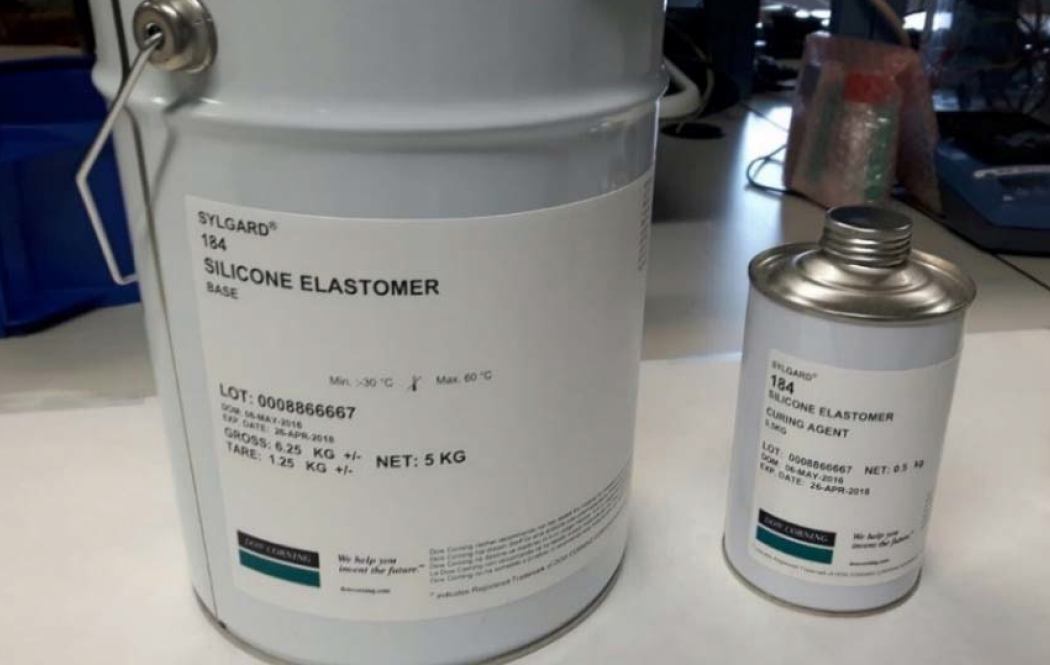
\includegraphics[width=0.75\textwidth]{./img/PDMS}
	\caption{PDMS: Elastómero y agente de cura.} \label{fig:pdms}
\end{figure}



\subsubsection{Proceso de fabricación del soporte físico}
%Elaboración
Para que sea más cómoda la explicación del proceso de elaboración del prototipo se divide este en tres partes: modelado 3D, fabricación del guante y montaje de prototipo completo.

\begin{itemize}
	\item \textbf{Modelado 3D - Configuración 3D}
	
	Esta actividad comprende el diseño del molde con el que se fabrica el guante y de la caja contenedora de todo el cableado.
	Para poder producir el guante de PDMS es necesario tener un molde donde verter la disolución para darle la forma deseada. Gracias a las versatilidad de diseño que ofrece la impresión 3D se realiza con este proceso de manufactura el molde (véase figura \ref{fig:molde}). 
\begin{figure}[H]
	\centering
	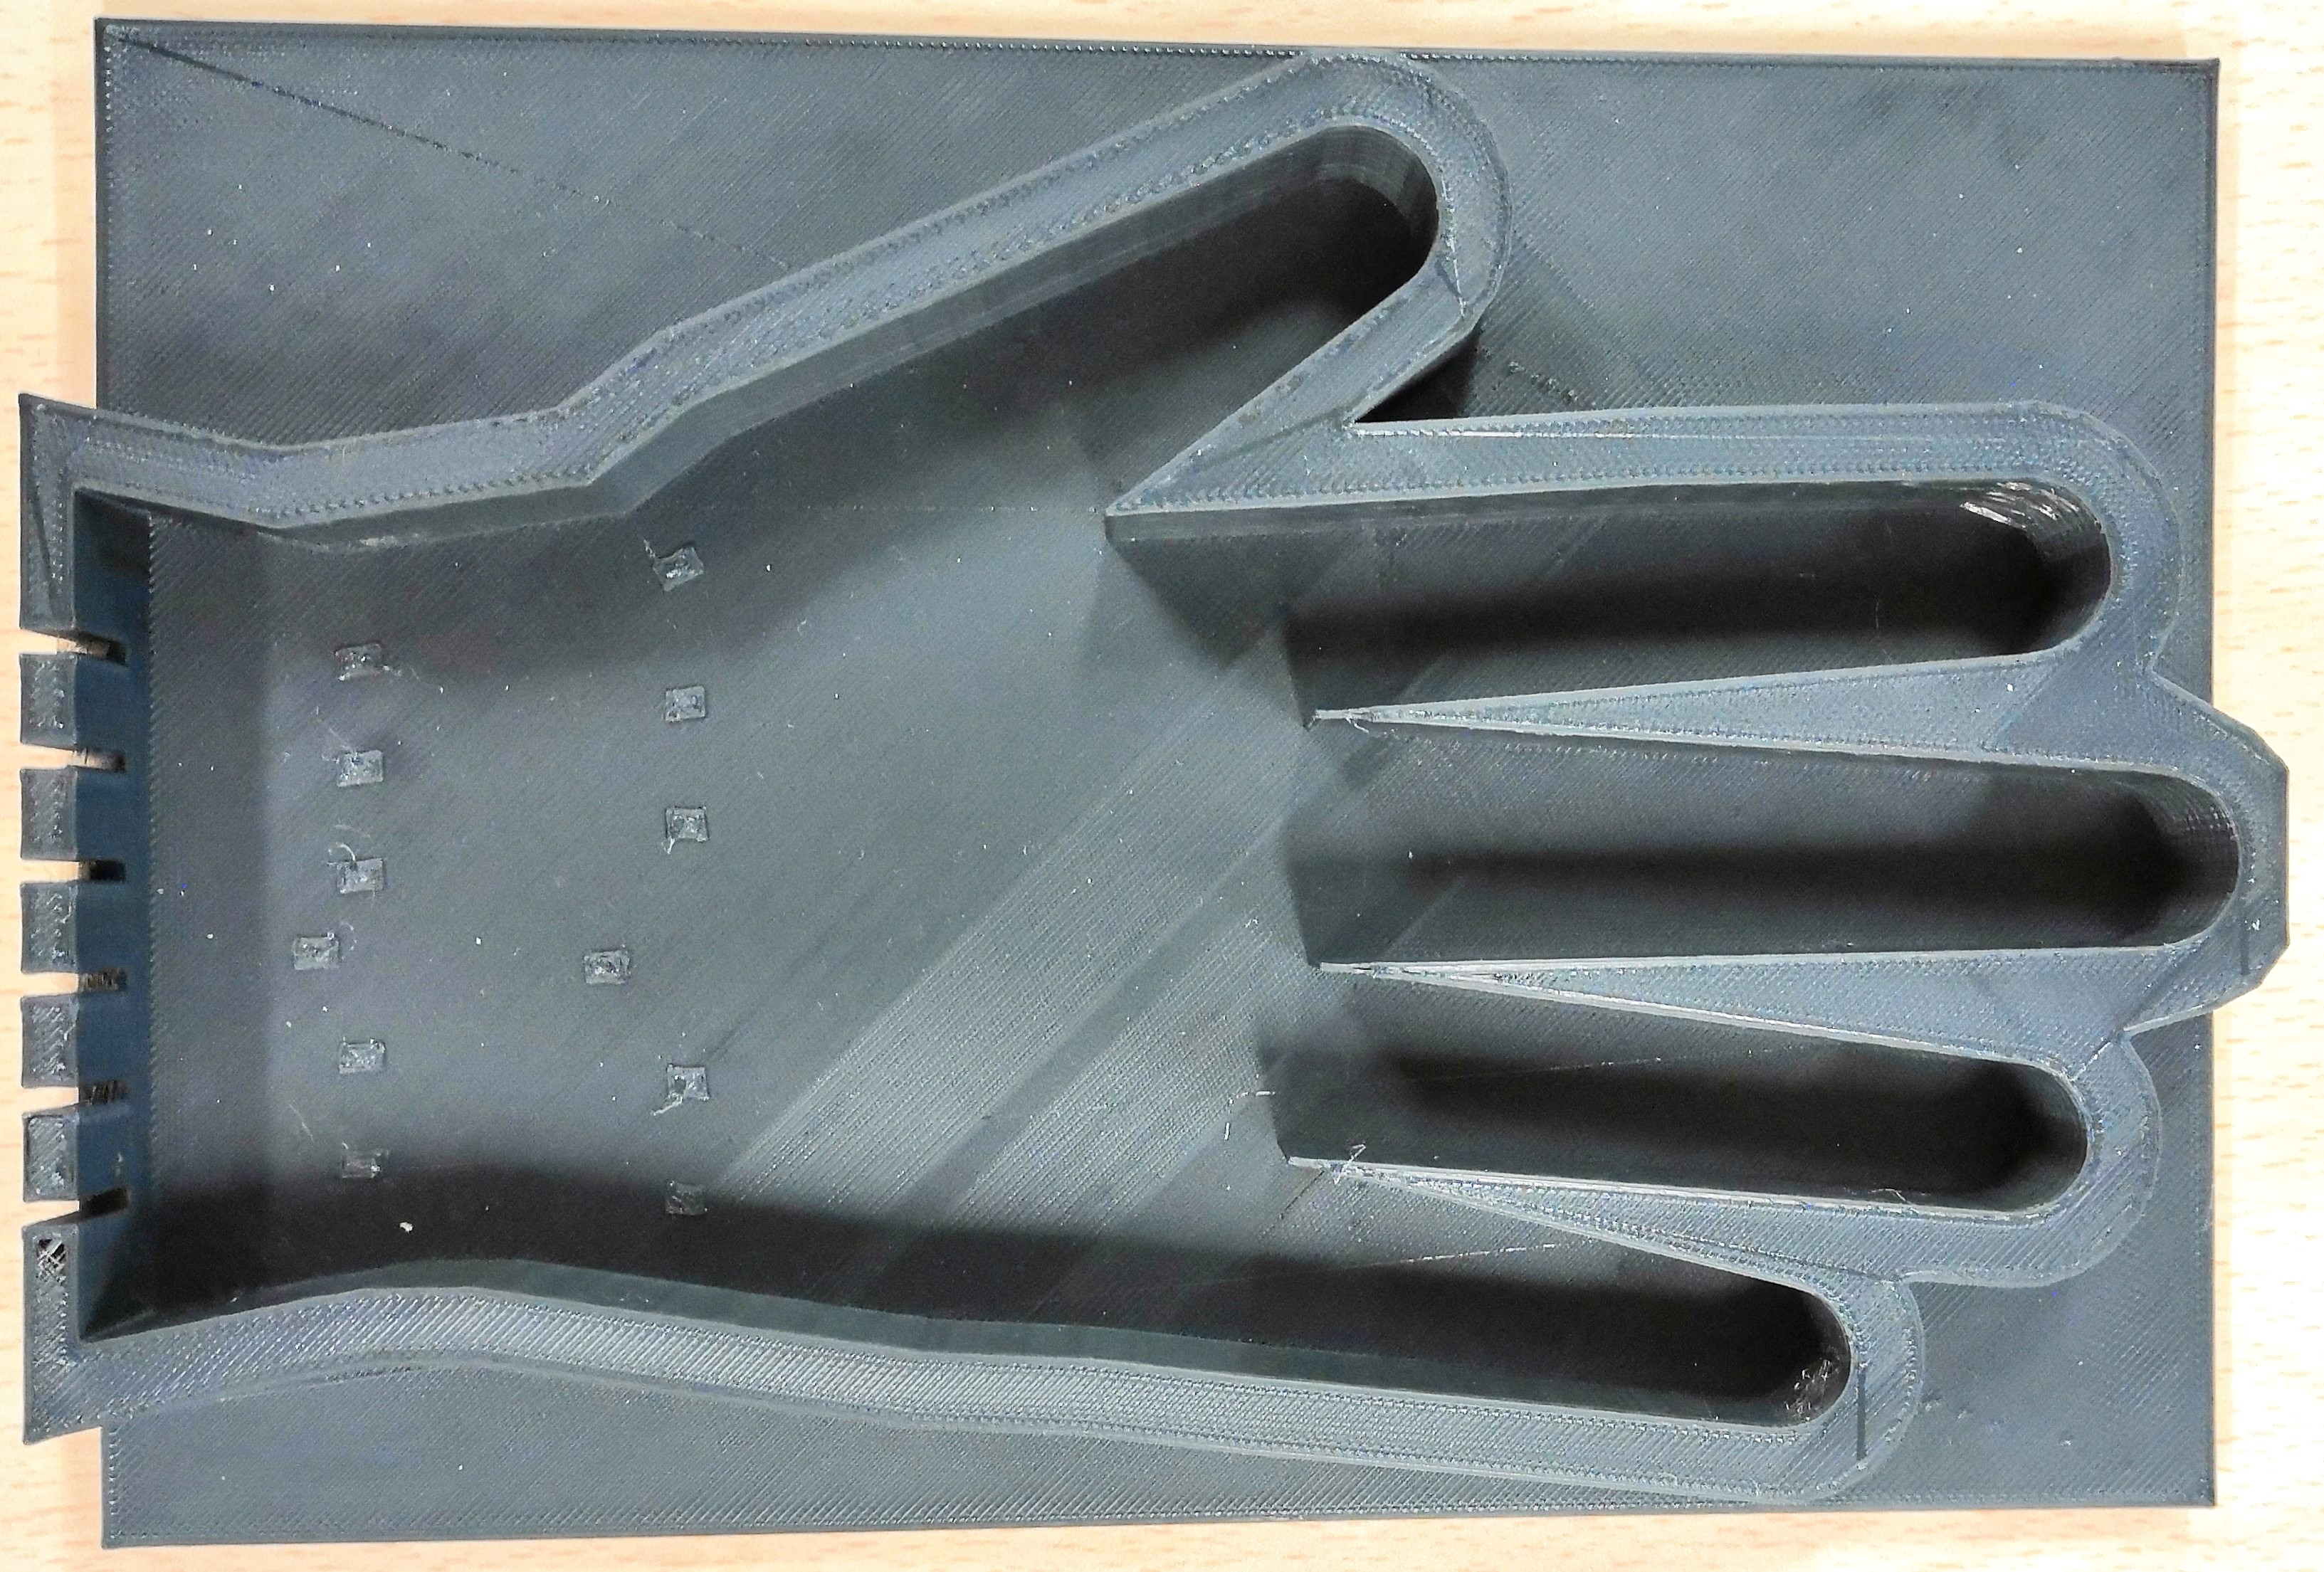
\includegraphics[width=0.5\textwidth]{./img/molde1}
	\caption{Molde} \label{fig:molde}
\end{figure}

	
 
	\item \textbf{Fabricación del guante}
	
	Para el proceso de fabricación del guante se necesitan ..................
	
	\begin{enumerate}
		\item Preparar mezcla PDMS (35g de polímero y 3.5g de agente de curación). Primero el
		elastómeto y después agente de curación.
		\item Revolver la mezcla durante al menos 4 minutos.
		\item Se deposita el PDMS y se colocan las fibras en el molde
		\item Se introduce en un horno de vacío para eliminar las burbujas durante 20 minutos, sin aplicar
		temperatura.
		\item Meter el molde en el horno (4h y media a $-55\,^{\circ}\mathrm{C}$). Dejar un poco más.
		\item Desmoldar.

	\end{enumerate}
	
	
	\item \textbf{Montaje completo}
	
	asdf
	
\end{itemize}

asdf





\begin{table}[H] %BORRAR
	\centering
	\begin{tabular}[t]{|c|}
		\hline
		\textbf{\textcolor{rositaoscuro}{BORRAR}} \\
		\hline
		longitudes de onda del guante de fibras cortas\\
		\hline
	\end{tabular}
	\begin{tabular}[t]{|r|c|}
		\hline
		 & Longitud de onda del sensor\\
		\hline
		\hline
		Dedo pulgar & 1512 nm \\
		\hline
		Dedo índice & 1520 nm \\
		\hline
		Dedo corazón & 1528 nm \\
		\hline
		Dedo anular & 1536 nm \\
		\hline
		Dedo meñique & 1544 nm \\
		\hline
		Muñeca & 1556 nm \\
		\hline
	\end{tabular}
	\caption{Tabla longitud de cada sensor FBG}
	\label{tabla:medidas 80 cm}
\end{table}
%-- Hasta aquí borrar la tabla.


\begin{table}[H]
	\centering
	\begin{tabular}[t]{|r|c|}
		\hline
		& Longitud de onda del sensor\\
		\hline
		\hline
		Dedo pulgar & 1532 nm \\
		\hline
		Dedo índice & 1548 nm \\
		\hline
		Dedo corazón & 1576 nm \\
		\hline
		Dedo anular & 1568 nm \\
		\hline
		Dedo meñique & 1560 nm \\
		\hline
		Muñeca & 1541.26 nm \\
		\hline
	\end{tabular}
	\caption{Tabla longitud de cada sensor FBG}
	\label{tabla:medidas 80 cm}
\end{table}

Para determinar la valid


\subsubsection{Funcionamiento}
asdf

\begin{figure}[H]
	\centering
	\includegraphics[width=1\textwidth]{./img/interfazSM}
	\caption{Interfaz del programa de labview.}
	\label{fig:interfaz}
\end{figure}

%------IIIIIIMMMMMMUUUUUU------
\section{Solución con sensores IMU}
\label{sec:IMU3}
asdf

\subsection{Marco conceptual}
\label{sec:mc3IMU}
asdf

\subsection{Desarrollo del prototipo}
\label{sec:prot3IMU}
asdf

\subsubsection{Materiales}
asdf


\subsubsection{Elaboración/Proceso de fabricación}
asdf

\subsubsection{Funcionamiento}
asdf




\section{---------------}

ME PLENTEO LA POSIBILIDAD DE DIVIDIR EL CAPITULO 3 EN CAPITULO 3 Y 4.


----------------------------------------------------------------------------------------------------------------------------------------------------------------------------------------------------------------------------------------------------------------------------------------------------------------------------------------------------------------------------------------------------------------------------------------------------------------------------------------------------------------------------------------------------------------------------------------------------------------------------------------------------------------------------------------------------------------------------------------------------------------------------------------------------------------------------------------------------------------------------------------------------------------------------------------------------------------------------------------------------------------------------------------------------------------------------------------------------------------------------------------------------------------------------------------------------------------------------------------------------------------------------------------------------------------------------------------------------------------------------------------------


\section{---------------}















En este capítulo se detalla la metodología empleada para el diseño del sistema adaptado al contexto en el que se aplica. Se describe cada uno de los componentes que forman parte del sistema de medición así como el procesado posterior de los datos para obtener la distancia entre pasos(Matlab\textsuperscript{\textregistered}). En el diseño intervienen sensores inerciales (Xsens Technologies B.V, The Netherlands) y se propone el diseño de un sensor de ultrasonido de bajo coste basado en la tecnología Arduino. 


\section{Sistema de medida}
En la Figura \ref{fig:esquema} aparece representado un esquema general de la metodología empleada. Mediante el sensor de ultrasonidos se obtiene la distancia D1 y con los sensores inerciales se obtiene la distancia D2 aplicando a cada una de las señales el procesado que se detallará en posteriores apartados.


Por tanto, el diseño del sistema puede descomponerse en dos niveles de jerarquía  (ver Figura \ref{fig:esquemaniveles}). El primero de ellos, a más bajo nivel, es el diseño del sensor de ultrasonidos y la obtención de las señales necesarias para el cálculo de cada una de las distancias de ambos sensores. El segundo de los niveles es el correspondiente al de la sincronizcación y post-procesado de los datos para determinar la distancia entre pasos.

 Con el  post-procesado de las señales obtenidas por cada uno de los sensores se obtendrán las distancias D1 y D2 que permitirán el cálculo de la distancia objetivo mediante la ecuación \ref{eq:distancia} (Teorema de Pitágoras).

\begin{equation}\label{eq:distancia}
Dist.sep.pasos = \sqrt{D1^2 + D2^2}
\end{equation}


En los siguientes apartados se especifican cada uno de los componentes que intervienen en el sistema. 
\section{Sensores inerciales}
\subsection{Principio de funcionamiento}

Un sistema de referencia inercial se trata de un sistema de referencia regido por las leyes de movimiento de Newton. Por tanto, un sensor capaz de medir valores respecto a dicho sistema de referencia es lo que se conoce como un sensor inercial.

Una unidad inercial o IMU (Inertial Magnetic Unit) es un dispositivo que se compone de tres giróscopos (para determinar la orientación), tres acelerómetros y un reloj que permite asignar tiempo a los valores medidos por los sensores inerciales. Dichas unidades inerciales presentan tres ejes y cada uno de ellos presenta un acelerómetro y un giróscopo.

Por tanto, la información que se recoge de las unidades inerciales son aceleraciones lineales, velocidades angulares y tiempo común para los tres ejes que llevan dicha información de aceleración y velocidad angular (ver Figura \ref{fig:Imu}). 


El tiempo requerido para la implementación del sistema de medida puede influir en la marcha de los pacientes y por tanto en la obtención de los parámetros \cite{begona}. Los sensores inerciales utilizados permiten realizar las mediciones de una manera sencilla y rápida lo cual resulta beneficioso en el contexto ambulatorio tanto para los pacientes como para el personal sanitario



\subsection{Sensores inerciales propuestos}
Los sensores inerciales utilizados para el sistema son el modelo MTw Awinda (Xsens Technologies B.V, The Netherlands) pueden verse representados en la Figura \ref{fig:sensor_XSENS}



Su tamaño es de 47 x 30 x 13mm y 16g de peso por lo que puede definirse como un sistema compacto y ergonómico que será de utilidad para el sistema propuesto en este trabajo. Dispone de unas bandas de sujeción que permiten colocar el sensor en el lugar necesario y por tanto dota de versatilidad al diseño. 

Además, se incluye un software de captura que resultará útil para obtener las señales para su posterior procesado. La comunicación de los sensores con el software emplea un protocolo propietario que aparece representado en la Figura \ref{fig:protocolo}.

	
\section{Sensor de ultrasonido}

\subsection{Principio de funcionamiento}
Un sistema de ultrasonidos tiene como principio de funcionamiento el fenómeno físico por el cual recibe ese nombre, las ondas de ultrasonidos.

Se envía un pulso de 40 KHz que incide sobre un obstáculo y se recibe con un retardo que se corresponde con el tiempo que tarda la onda desde que se envía hasta que se recibe, es decir el Time of Flight" (ToF). Por tanto, puede hallarse la distancia mediante la 

	 En la Figura \ref{fig:ultr} se observa dicho funcionamiento.

La distancia entre dos puntos puede hallarse mediante la ecuación \ref{eq:dis_ult}
	\begin{equation}\label{eq:dis_ult}
	D = (ToF/2)V_{sonido}
	\end{equation}
	
Una alternativa al sistema de ultrasonidos es usar la tecnología de infrarrojos. Su principal ventaja es su rápida respuesta y por ello resulta beneficioso para aplicaciones en tiempo real como pueden ser los sensores de proximidad. La principal desventaja es que presentan no linealidades procedentes de su dependencia con la superficie de reflexión. Es necesario un conocimiento a priori de las características de dispersión, absorción etc. del material sobre el que incide la onda emitida para poder realizar una medida de distancia correcta. 

Teniendo en cuenta las características de ambos sensores, se decidió que el sensor más apropiado para la aplicación clínica de este trabajo es el sensor de ultrasonidos, ya que su coste no es elevado y su resolución y su latencia son aceptables. Se ha descartado el uso de un sensor de infrarrojos, por un lado, porque la velocidad no es un factor crítico y por otro lado, realizar una medida de distancia con este tipo de sensores supone la necesidad de conocer a priori el material del calzado de cada paciente o añadir una superficie con un material concreto en uno de los zapatos del paciente lo cual hace que el diseño resulte menos ergonómico. Finalmente añadir que aunque existen sensores de infrarrojo basados en la medida de desfase que podrían utilizarse como sensores de distancia, su precio es realmente elevado para las características necesarias en este trabajo \cite{infra}
	

\subsection{Sensor de ultrasonido propuesto}\label{su}

	El principal objetivo en el diseño del sensor es optimizar el compromiso entre bajo coste y precisión. En la Figura \ref{fig:sensor_ultrasonido} puede verse el prototipo del sensor. Este primer prototipo está compuesto por un sensor de ultrasonidos HC-SR04 (1), un módulo Bluetooth (2) para el envío de datos a un PC, una placa Arduino UNO (3) para el procesado de la información del sensor, y la alimentación mediante una pila recargable de 9V (4) para dotar de autonomía al sistema.

 \begin{figure}[H]
 	\centering
 	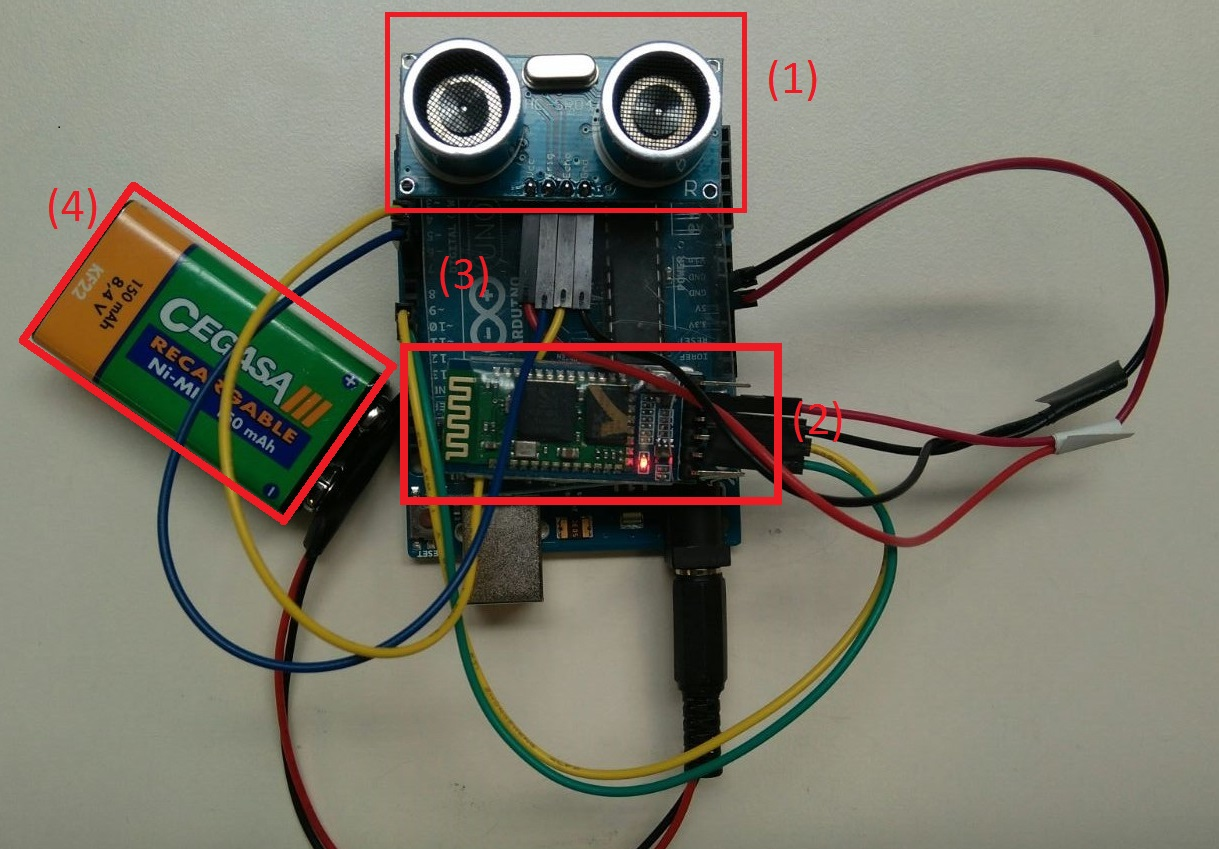
\includegraphics[width=0.7\textwidth]{./graphics/sensor}
 	\caption{Prototipo de sensor de ultrasonidos} \label{fig:sensor_ultrasonido}
 \end{figure}

	\subsubsection{Conexionado del sensor}
		El conexionado del prototipo (apartado \ref{su}), aparece representado de manera esquemática en la Figura \ref{fig:conexionado} con el fin de clarificar las conexiones. En un futuro diseño más compacto, la placa utilizada, así como algunos de los componentes, serán modificados manteniendo el enfoque de bajo coste, ergonomía y precisión. Por ello las conexiones podrán ser modificadas según sea necesario.
		
		 
		\begin{figure}[H]
			\centering
			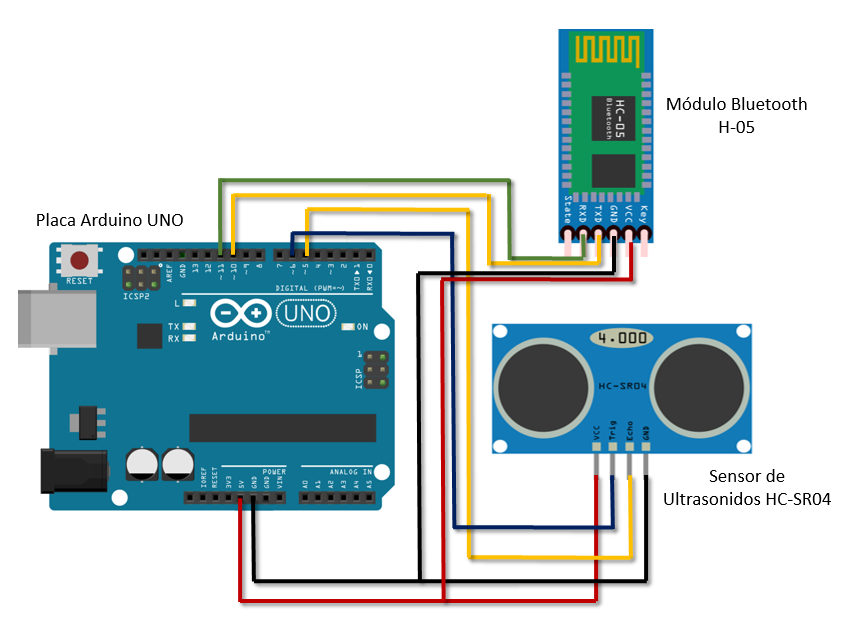
\includegraphics[width=0.7\textwidth]{./graphics/conexionado}
			\caption{Esquema de conexión del sensor de ultrasonido} \label{fig:conexionado}
		\end{figure}
		
	\subsection{Comunicación del sensor}
	
		\subsubsection{Bluetooth}
		
		Para el envío de la información de distancia desde la placa Arduino hasta el PC donde se van a procesar los datos, se ha elegido el módulo comercial Bluetooth H-05 que aparece representado en la Figura \ref{fig:bluetooth}.
		
	
			 \begin{figure}[H]
			 	\centering
			 	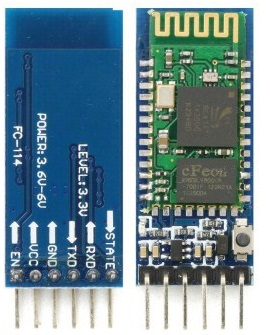
\includegraphics[width=0.25\textwidth]{./graphics/bluetooth}
			 	\caption{Módulo Bluetooth HC-05} \label{fig:bluetooth}
			 \end{figure}
			 
		Dicho módulo se comunicará con un dongle USB 4.0 en el PC ya que éste no dispone de interfaz Bluetooth de serie (ver Figura \ref{fig:dongle}). Además es compatible con estándares anteriores (2.0, 3.0) por lo que resulta apropiado para el diseño.
		
		
		\begin{figure}[H]
			\centering
			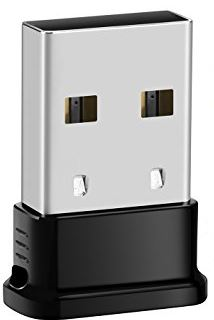
\includegraphics[width=0.15\textwidth]{./graphics/dongle}
			\caption{Dongle Bluetooth 4.0 WhiteLabel} \label{fig:dongle}
		\end{figure}
			
		\subsubsection{Software de captura}
		
		En este trabajo se ha diseñado un software de captura (Figura \ref{fig:software}) para la obtención de los datos de distancia suministrados por el sensor.
		

		Las funcionalidades principales de este software son:
		\begin{enumerate}
				\item Creación del interfaz Bluetooth para la comunicación con Matlab. 
				\item Representación de los datos recogidos en tiempo real.
				\item Posibilidad de guardar los datos en un archivo.
				\item Posibilidad de cargar un archivo y representarlo offline.
		\end{enumerate}
	
		
\section{Procedimiento de medida}		

\subsection{Set-up de medida}
Para demostrar la viabilidad del sistema en cuanto a su capacidad para medir la distancia de separación entre pasos,se proponen dos set-ups que consisten en establecer unas marcas en el suelo a una distancia conocida para así, una vez realizado el procesado de las señales, poder determinar si los resultados son correctos. El primer set-up consta de una medida de paso de 43 cm (ver Figura \ref{fig:setup_43}) y el segundo para una de 80.5 cm (ver Figura  \ref{fig:setup_80} ). 

\begin{figure}[H]
	\centering
	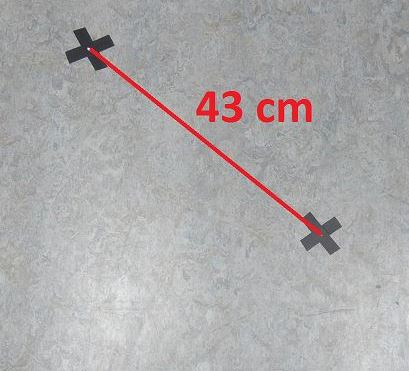
\includegraphics[width=0.55\textwidth]{./graphics/setup_43}
	\caption{Set-up de medida de un paso de 43 cm} \label{fig:setup_43}
\end{figure}

\begin{figure}[H]
		\centering
		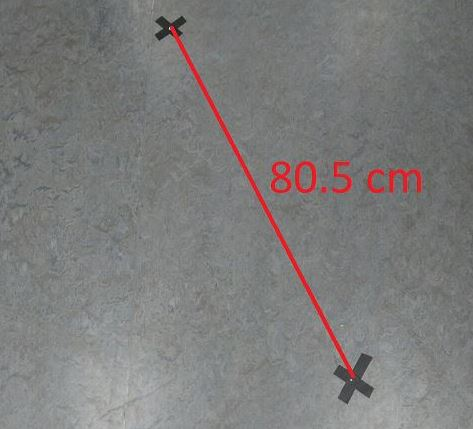
\includegraphics[width=0.55\textwidth]{./graphics/setup_80}
		\caption{Set-up de medida de un paso de 80.5 cm} \label{fig:setup_80}
\end{figure}
	
Este montaje permitirá el poder medir un la distancia de un paso para verificar que el tanto el funcionamiento como el procesado con correctos. Se dejará como línea futura el poder realizar el procesado de forma automática y para varios pasos. Para realizar las medidas se ha colocado un sensor inercial en cada pie y el sensor de ultrasonidos en el tobillo según se representa en la Figura \ref{fig:colocar} y \ref{fig:paso}. 
\begin{figure}[H]
	\centering
	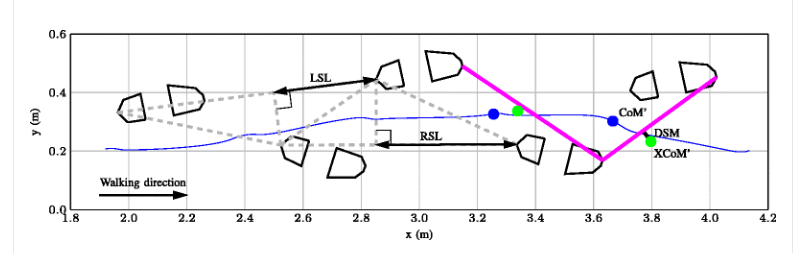
\includegraphics[width=0.55\textwidth]{./graphics/Medida}
	\caption{Colocación de los sensores para la medida} \label{fig:colocar}
\end{figure}
\begin{figure}[H]
	\centering
	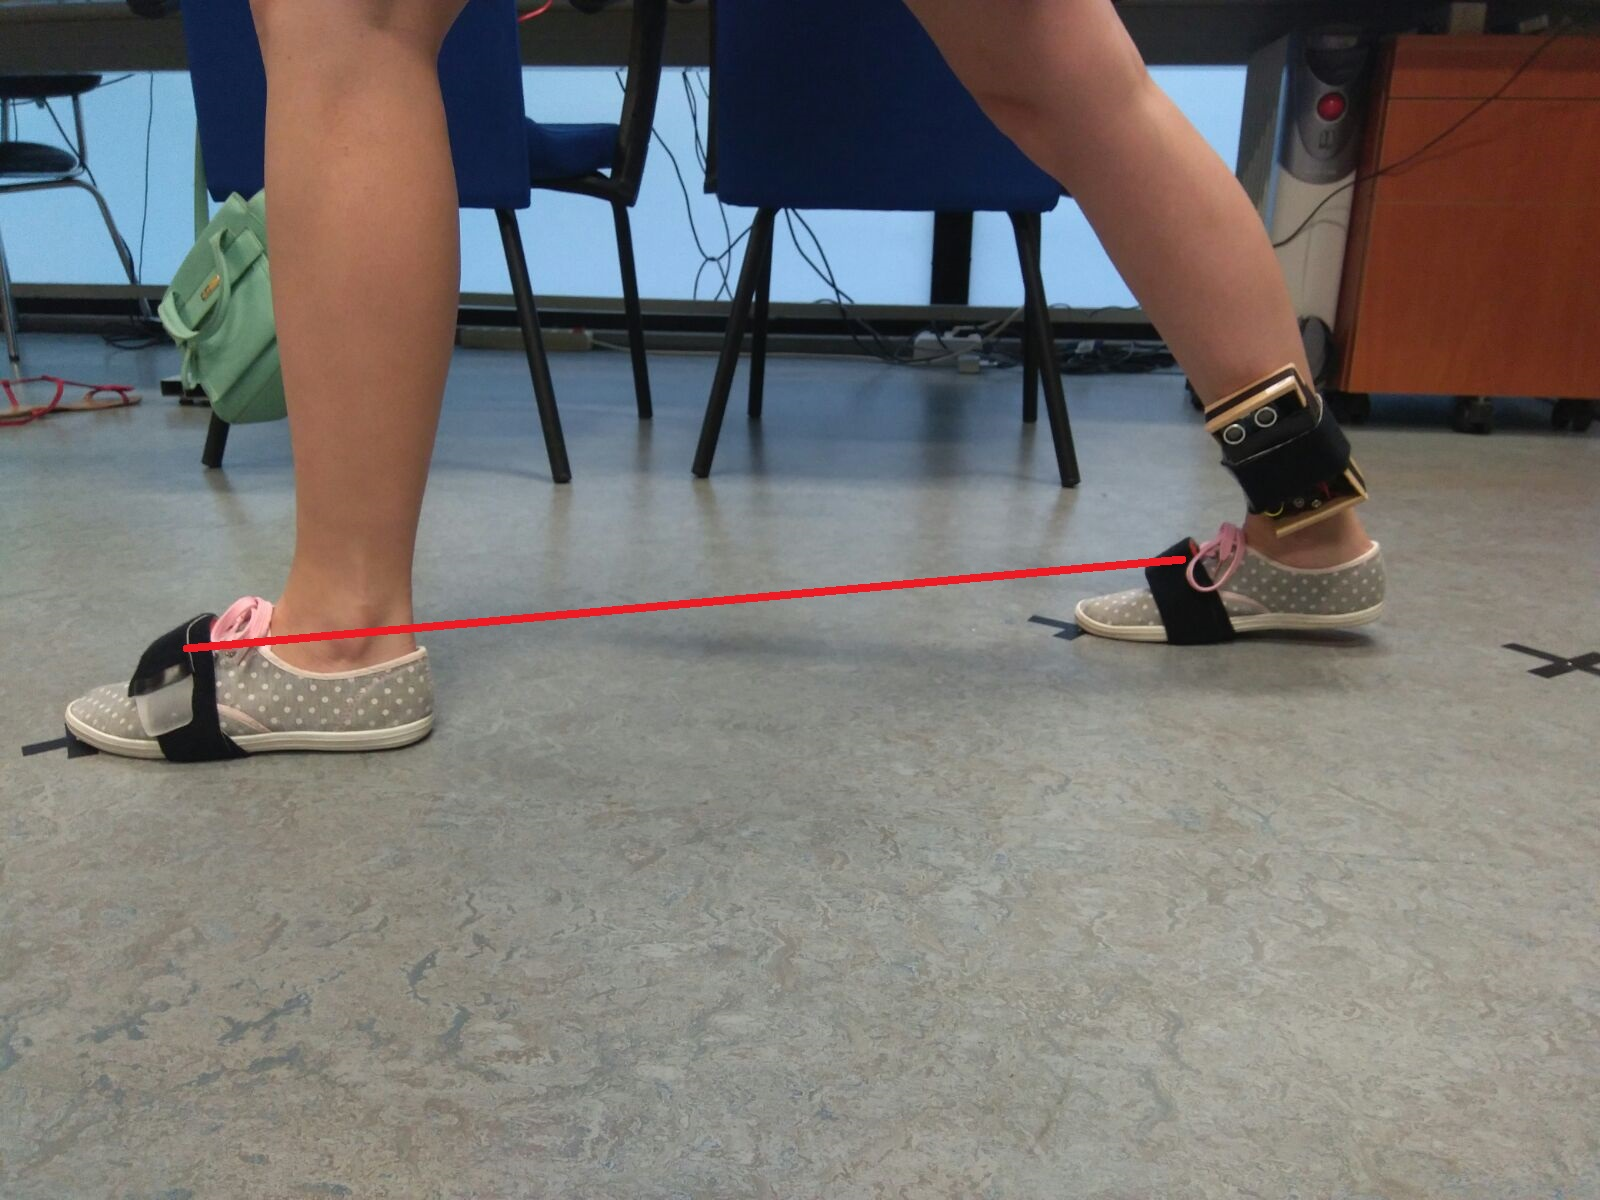
\includegraphics[width=0.65\textwidth]{./graphics/paso}
	\caption{Ejemplo de paso para la medida} \label{fig:paso}
\end{figure}


\subsection{Captura de datos}

Para llevar a cabo la medida se colocará un sensor inercial en cada pie y el sensor de ultrasonidos en uno de ellos. A continuación, se capturarán los datos de los sensores inerciales mediante el software específico MTManager de Xsens y los datos del sensor de ultrasonido mediante el software realizado con MATLAB\textsuperscript{\textregistered} 


\subsection{Sincronización}
Una de las etapas clave del diseño del sistema a tiempo real es el de la sincronización de ambos sensores. En este trabajo, para una demostración de funcionamiento, el procesado de las señales de ambos sensores se realizará por separado de forma que se pueda demostrar el funcionamiento del sistema y se dejará como línea futura de investigación la sincronización. 

Se pretende conseguir una lectura de los datos del sensor de ultrasonido en el PC con un tiempo de muestreo constante. En este punto del trabajo se encuentran dificultades con la forma en que Matlab lee los datos. Los datos enviados por el sensor son constantes pero la lectura hace ese tiempo variable. Si se consigue un tiempo constante, mediante procesados como la interpolación podría sincronizarse con los sensores inerciales. Además, debido a que se utilizan dos programas de captura, es necesario establecer un inicio que se considere como principio tanto para las señales de los sensores inerciales como el de ultrasonidos. 


\subsection{Obtención de distancia}
Para la obtención de la distancia de separación entre pasos existen tres scripts realizados con la herramienta software Matlab\textsuperscript{\textregistered}

Mediante un software en Matlab\textsuperscript{\textregistered} se cargan las señales y se realiza el post-procesado para obtener cada una de las distancias que van a permitir la obtención de la distancia de separación entre pasos.

Se procesará el cálculo de las distancias deseadas de los sensores inerciales y del de ultrasonido y dichas informaciones se utilizarán para la obtención de la distancia de separación entre pasos.

\subsubsection{Sensores inerciales}

	
	Para la obtención del dato de distancia a partir de las señales proporcionados por los sensores inerciales es necesario tener en cuenta que la distancia se recorre en el plano en el que se produce el avance, que es este caso es el plano XY.

Para obtener la posición en este plano a partir de la aceleración en los tres ejes XYZ proporcionada por los sensores inerciales, es necesaria una doble integración.Posteriormente se elimina la deriva existente en las señales debido a esta integración. A continuación se describen los cálculos realizados

\begin{itemize}
	
	\item{\textbf{Obtención de la velocidad}}
	
		Se realiza una primera integración de la aceleración en el eje X y en el eje Y de donde se obtiene la velocidad tal y como aparece en la Figura \ref{fig:vel_no_corr}
	 \begin{figure}[H]
	 	\centering
	 	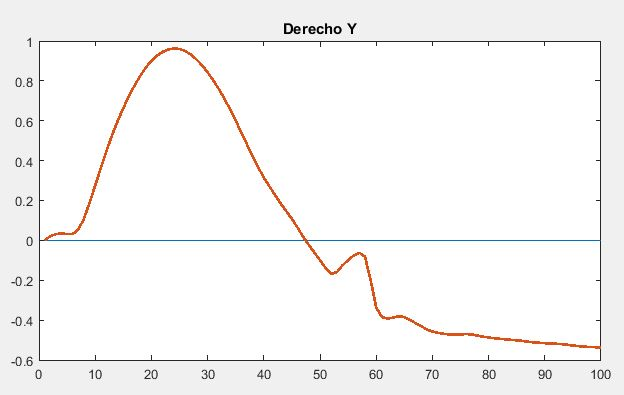
\includegraphics[width=0.81\textwidth]{./graphics/vel_no_corr}
	 	\caption{Ejemplo de deriva en la señal} \label{fig:vel_no_corr}
	 	
	 \end{figure}
 
	\item{\textbf{Obtención de la velocidad sin deriva}}	
	
En el instante de inicio y fin del paso, cuando el pie permanece apoyado, la velocidad debe ser cero.. Para lograr eliminar la deriva en la señal se propone utilizar la ecuación de la recta (color morado) que aparece en la Figura  \ref{fig:vel_no_corr_rect} . Dicha recta entre dos puntos A(a1, a2) y B(b1,b2) se difine mediante la ecuación \ref{eq:recta}
	
	\begin{equation}\label{eq:recta}
	y = (\frac{b_{2}-b_{1}}{a_{2}-a_{1}})*(x-a_{1})+b_{1}
	\end{equation}
	
	;donde:
	\begin{itemize}
		\item b2: coordenada y del último punto escogido (B)
		\item b1: coordenada x del último punto escogido (B)
		\item a2: coordenada x del primer punto escogido (A)
		\item a1: coordenada y del primer punto escogido (A)

	
	\end{itemize}


		 \begin{figure}[H]
		 	\centering
		 	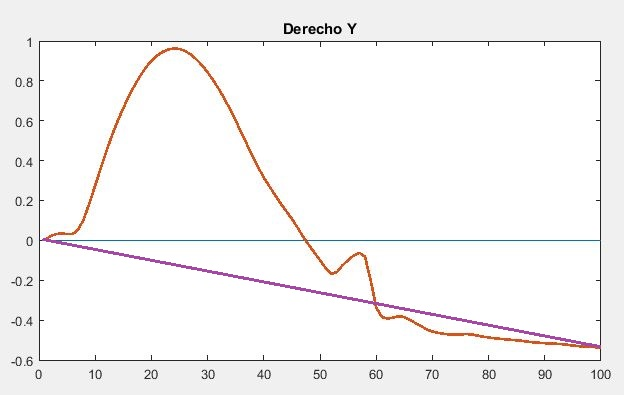
\includegraphics[width=0.8\textwidth]{./graphics/vel_no_corr_deriva}
		 	\caption{Recta para la corrección de la deriva} \label{fig:vel_no_corr_rect}
		 	
		 \end{figure}
De esta forma restando a la señal de velocidad la recta calculada, el resultado es el que aparece en la Figura \ref{fig:corregida} donde se representa la velocidad sin deriva.

	
		 \begin{figure}[H]
		 	\centering
		 	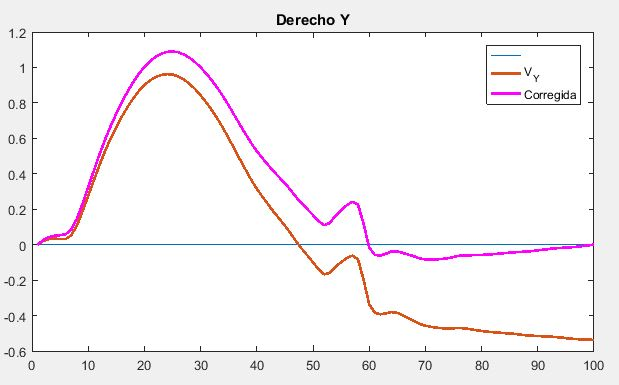
\includegraphics[width=0.8\textwidth]{./graphics/corregida}
		 	\caption{Ejemplo eliminación de la deriva} \label{fig:corregida}
		 \end{figure}


	\item{\textbf{Obtención de distancia D2 de sensores inerciales}}

	
	Una vez corregida la deriva en las velocidades X e Y de los sensores izquierdo y derecho en necesaria una segunda integración para hallar la posición en cada uno de los ejes. A continuación se representa la posición en el eje X con respecto al eje Y para calcular la distancia total en el plano XY (ver Figura \ref{fig:posi})
	\begin{figure}[H]
		\centering
		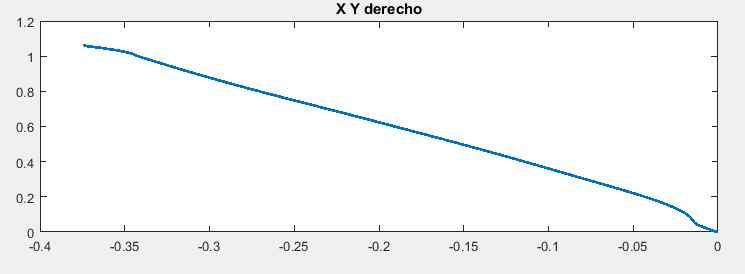
\includegraphics[width=1\textwidth]{./graphics/posi}
		\caption{Ejemplo eliminación de la deriva} \label{fig:posi}
		
	\end{figure}
	
	Para el cálculo de la distancia será necesario la eliminación de la deriva en la posición.
	
	La distancia (D2) ahora será la distancia entre los puntos inicial y final de la Figura \ref{fig:posi}, una vez corregida la deriva, que se calculará mediante la ecuación \ref{eq:pos}
		\begin{equation}\label{eq:pos}
		Distancia = \sqrt{(b_{1}-a_{1})^{2}+(b_{2}-a_{2})^{2}}
		\end{equation}
		\begin{equation}\label{eq:punto2}
			B = [b_{1},b_{2}]	
		\end{equation}
		\begin{equation}\label{eq:puntos1}
			A = [a_{1},a_{2}]
		\end{equation}
		;donde:
		\begin{itemize}
		\item b2: coordenada y del último punto escogido (B)
		\item b1: coordenada x del último punto escogido (B)
		\item a2: coordenada x del primer punto escogido (A)
		\item a1: coordenada y del primer punto escogido (A)
		\end{itemize}
\end{itemize}



\subsubsection{Sensor de ultrasonido}

	Previamente a la obtención de la distancia que se desea obtener usando el sensor de ultrasonido, se realiza una comprobación del correcto funcionamiento tanto del dispositivo como del envío de datos al PC vía Bluetooth. Inicialmente se realizan medidas con el sensor en estático. Para ello se propone el set-up de medida que aparece representado en la Figura  \ref{fig:ultrasonido}.
		
		 \begin{figure}[H]
		 	\centering
		 	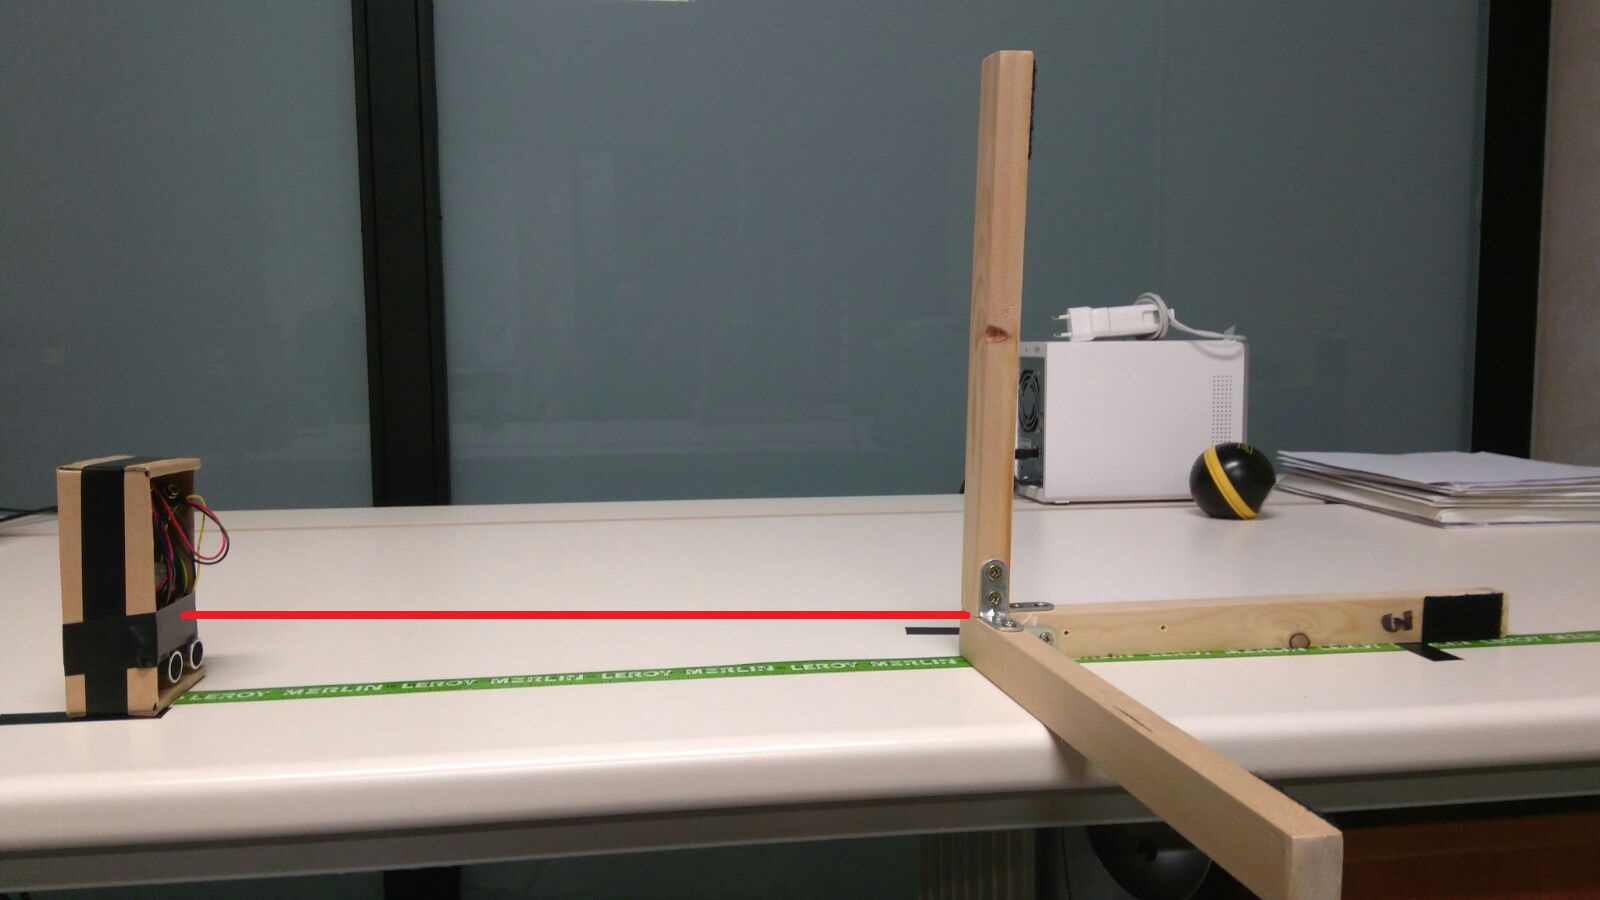
\includegraphics[width=0.95\textwidth]{./graphics/ultrasonido}
		 	\caption{Setup medida estática de sensor de ultrasonido}\label{fig:ultrasonido}
		 \end{figure}

Para estimar la precisión y el correcto funcionamiento del sensor se ha calculado el error absoluto y relativo de cada una de las medidas realizadas.

Una vez hecha dicha comprobación en estático, se añade al sistema de medida completo. Para ello se coloca el sensor en el tobillo y con el sensor orientado hacia la otra pierna (ver Figura \ref{fig:ultracoloc}).
		
	 \begin{figure}[H]
	 	\centering
	 	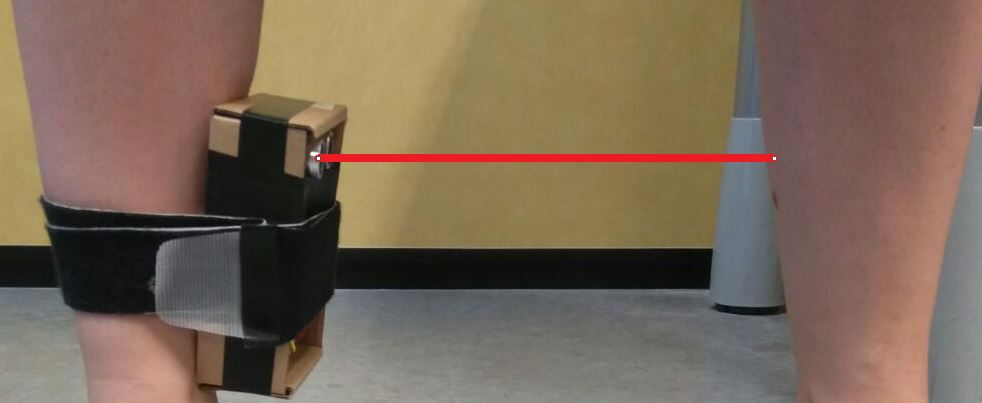
\includegraphics[width=0.8\textwidth]{./graphics/coloc_ultr}
	 	\caption{Colocación de sensor para medidas en dinámico} \label{fig:ultracoloc}
	 \end{figure}
				
		
\subsubsection{Obtención de distancia de separación entre pasos}

Una vez calculadas las distancias necesarias, se procede al cálculo de la distancia de separación entre pasos. En la Figura \ref{fig:sep} se representa dicho cálculo. La distancia D2 es la correspondiente al cálculo de la distancia con el sensor inercial izquierdo en este caso, la distancia D1 es la distancia calculada mediante el sensor de ultrasonido.
\begin{figure}[H]
	\centering
	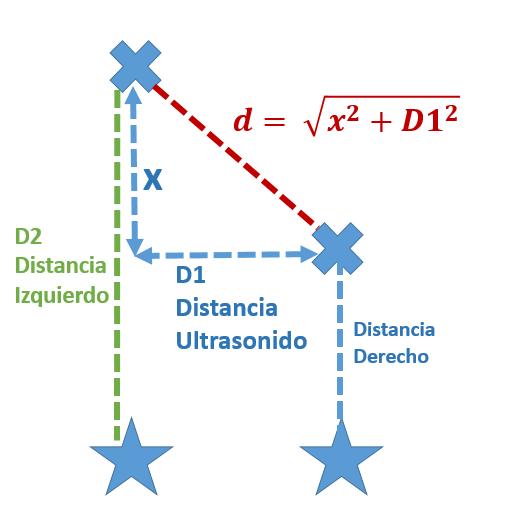
\includegraphics[width=0.8\textwidth]{./graphics/sep}
	\caption{Cálculo final de distancia de separación entre pasos} \label{fig:sep}
\end{figure}

Por tanto, para obtener X se utiliza la ecuación \ref{eq:x}
\begin{equation}\label{eq:x}
x = D2 - DistanciaDerecho
\end{equation}
En el caso de que el primero de los pasos se comenzase con el izquierdo la ecuación es la relativa a la DistanciaIzquierdo.

Para determinar la distancia, se utiliza por tanto, la ecuación \ref{eq:d}
\begin{equation}\label{eq:d}
d = \sqrt{x^{2}+D1^{2}}
\end{equation}